\section{Classifier Design}
\label{sec:ClasDes}
As stated in the introduction, a classifier had to be build for two different cases. For both cases, a similar design approach was used. \begin{enumerate}
	\item Investigate amount of data and use the theory to choose an initial representation method
	\item Train simple classifiers based on the chosen representation method
	\item Perform evaluation
	\item If the performance does not meet the requirements, go back to the theory
	\item If the performance meets the requirements, optimise the system
\end{enumerate}
This approach is visualised in figure \ref{fig:case_design}.
\begin{figure}[H]
	\centering
	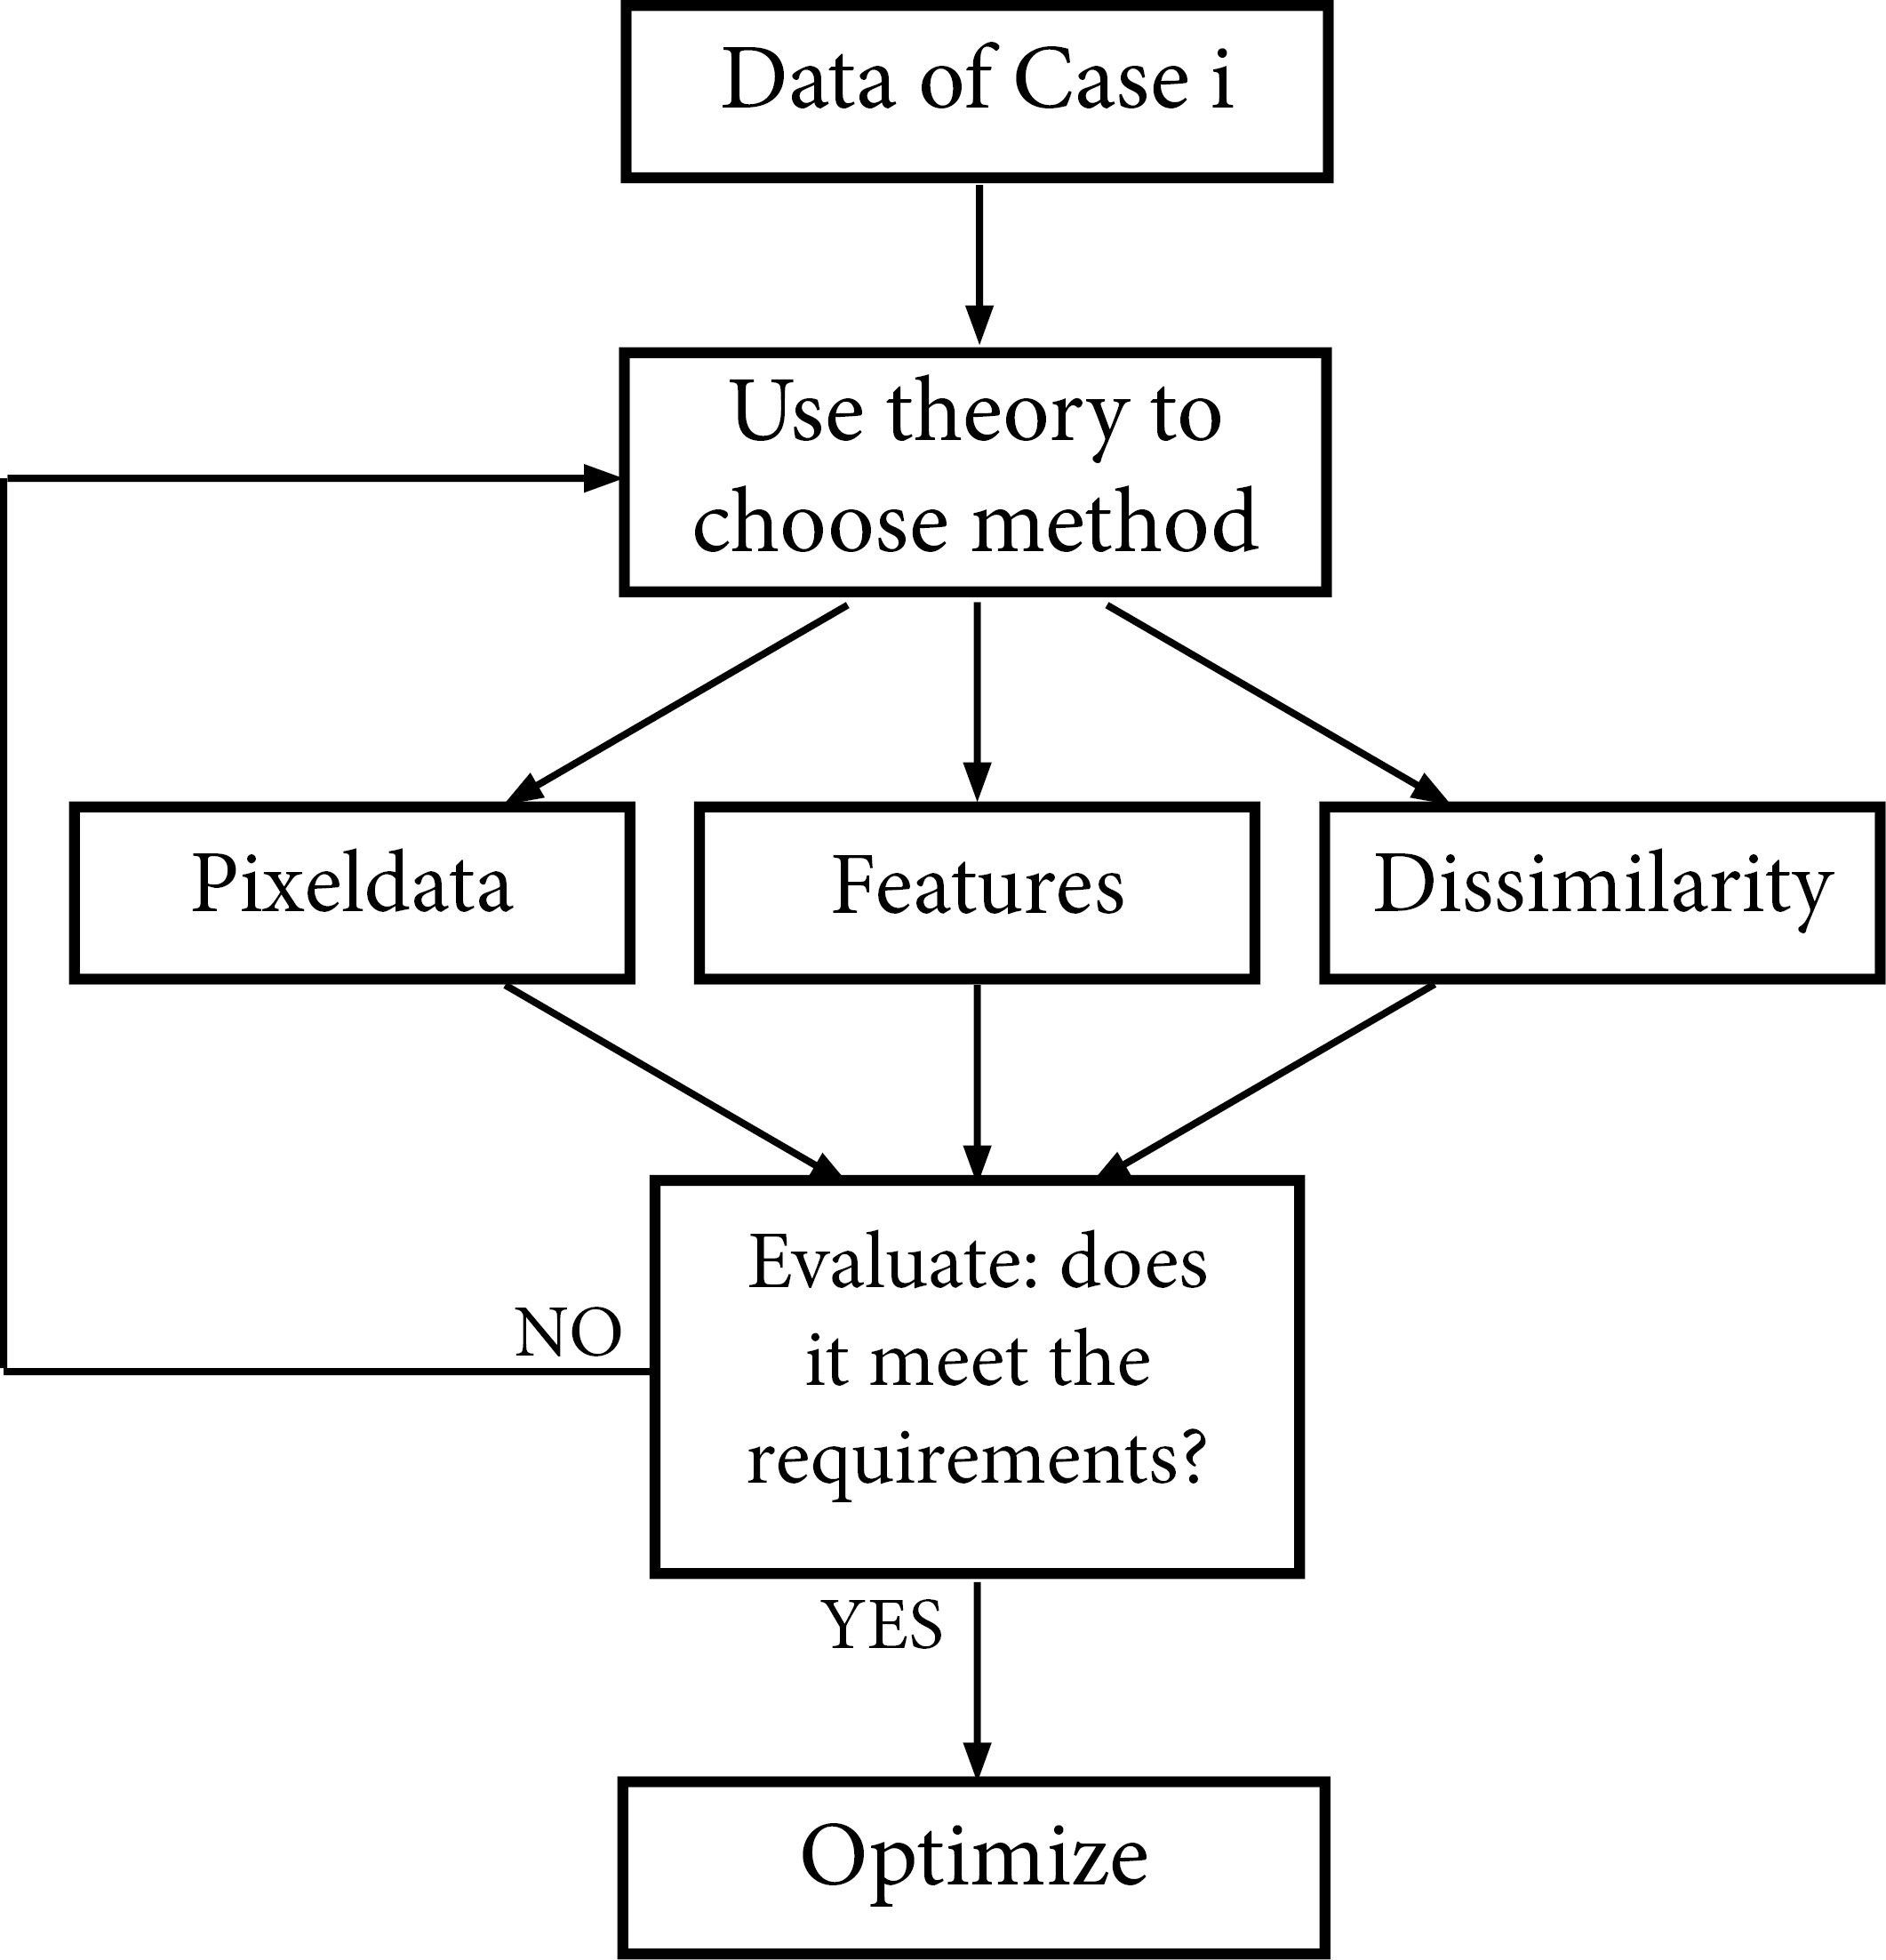
\includegraphics[scale=0.55]{images/Case_Design.jpg}
	\caption{Design-process to determine the best representation method for each of the two cases described in the Introduction.}
	\label{fig:case_design}
\end{figure}
\noindent The image processing described in chapter \ref{sec:ImPros} was kept the same for both cases, since it is a very subtle processing and will benefit all potential methods.

\subsection{Case 1}
\label{sec:Case1}
\textbf{Case Summary:} Design a system for training on all cheques at once. The system must be able to correctly classify the handwritten digits after being trained on at least 200 objects per class.\\
Smag

\subsection{Case 2}
\label{sec:Case2}
\textbf{Case Summary:} Design a system for training on each batch of cheques to be processed. The system must be able to correctly classify the handwritten digits after being trained on a maximum of 10 objects per class.\\
\\
\noindent The amount of data available in this case poses some restrictions. While a pixel-data representation worked very well in Case 1, it will have too little data to work with in this case.  
\\
\subsubsection*{Representation by Features}
To start out, features were chosen as the best representation for this case. The function \texttt{im\_features} from the prtools-toolbox was used to compute 14 different features of all the images in the pre-processed database. Because the this amount of features is relatively high compared to the amount of data that is used, some form of feature reduction needs to by applied. MatLab's forward feature selection (\texttt{featself}) was used initially to get a sense for the features that should be used and the features that could be omitted. This was done for four cases; with and without scaling of the data, and with and without implementing a separate test-set in the \texttt{featself} function. The resulting performance can be seen in figure \ref{fig:featsel_perf}
\begin{figure}[H]
	\centering
	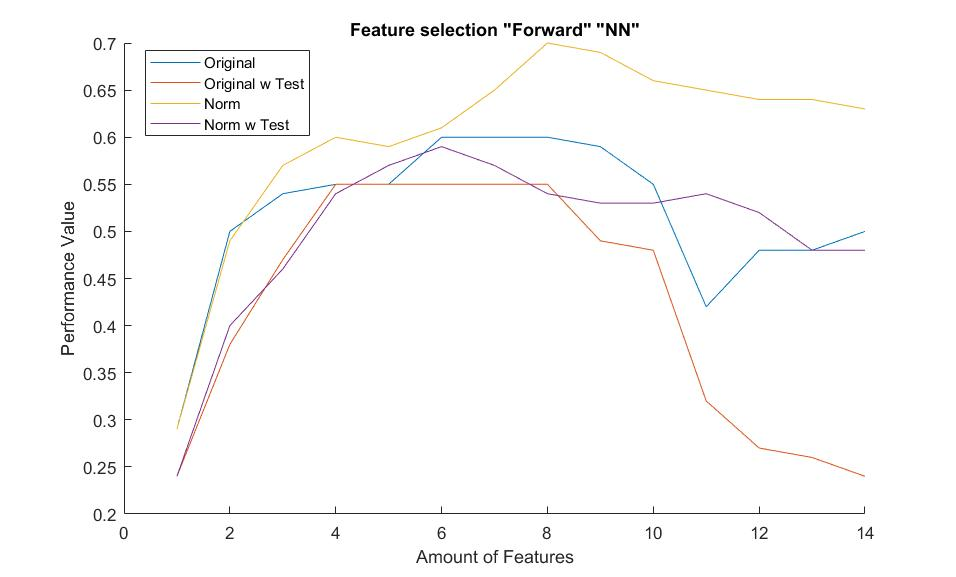
\includegraphics[scale=0.45]{images/featsel_perf.jpg}
	\caption{Performance of features selected by forward feature selection. Both scaling and non-scaling, and with or without test-set are shown.}
	\label{fig:featsel_perf}
\end{figure}
\noindent As can be seen in the figure, there are a lot of differences however between the different parameters. There appears to be an optimal amount of features however, somewhere between 4 and 12. In order to get a better grip on which features to use, a brute force approach was taken. Each possible combination between 3 and 14 features was used for an error-calculation (using the \texttt{testc}  function of PRTools) of four different classifiers (Fischer's Classifier, Linear Classifier, Nearest Mean Classifier and a Nearest Mean Classifier trained on normalized data). After running this setup overnight, the following results were obtained: (see figure \ref{fig:feat_bf_error}).
\begin{figure}[H]
	\centering
	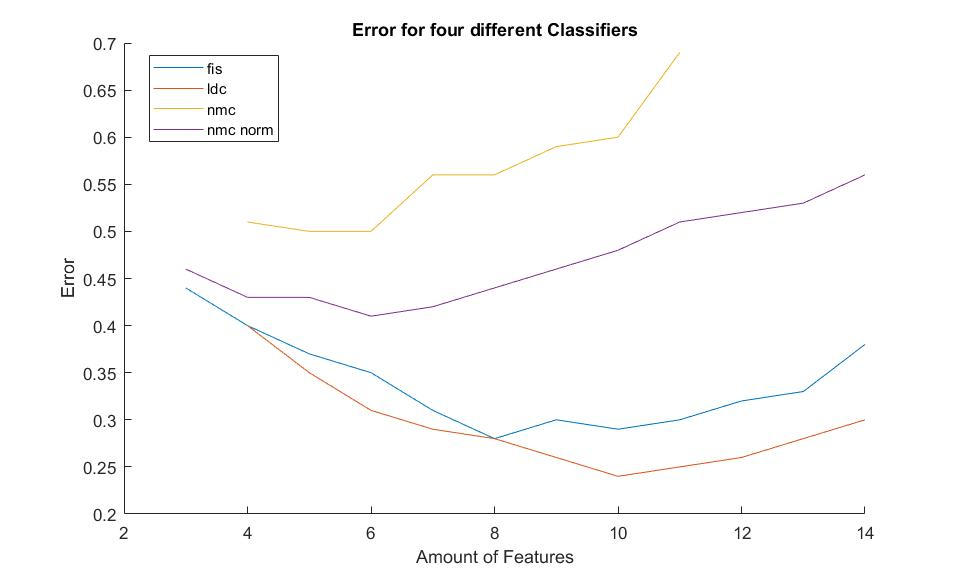
\includegraphics[scale=0.45]{images/feat_bf_error.jpg}
	\caption{Error of different combinations of features for four different trained classifiers; Fischer's (\texttt{fischerc}), Linear Bayes-Normal (\texttt{ldc}), Nearest Mean (\texttt{nmc}) and a normalised version of Nearest Mean.}
	\label{fig:feat_bf_error}
\end{figure}
\noindent This figure also clearly suggests an optimal combination of features. It also shows that the Linear Classifier will probably perform best, although even its best error is not under the 25 percent yet. \\
Next, for the LDC classifier only, each possible combination of 10 features was tested. In figure \ref{fig:feat_jumps} the error of each of these combinations can be seen. Very noticeable are the large drops and jumps in the graph, visualised with the orange line below it. after close inspection of the used features at these points, it was discovered that every increase in error corresponded to the same four features being added, namely 'Convex Area', 'Conves Hull', 'Convex Image' and 'Eccentricity'. It was decided to omit these features, leaving the final dataset with the desired amount of 10 features.
\begin{figure}[H]
	\centering
	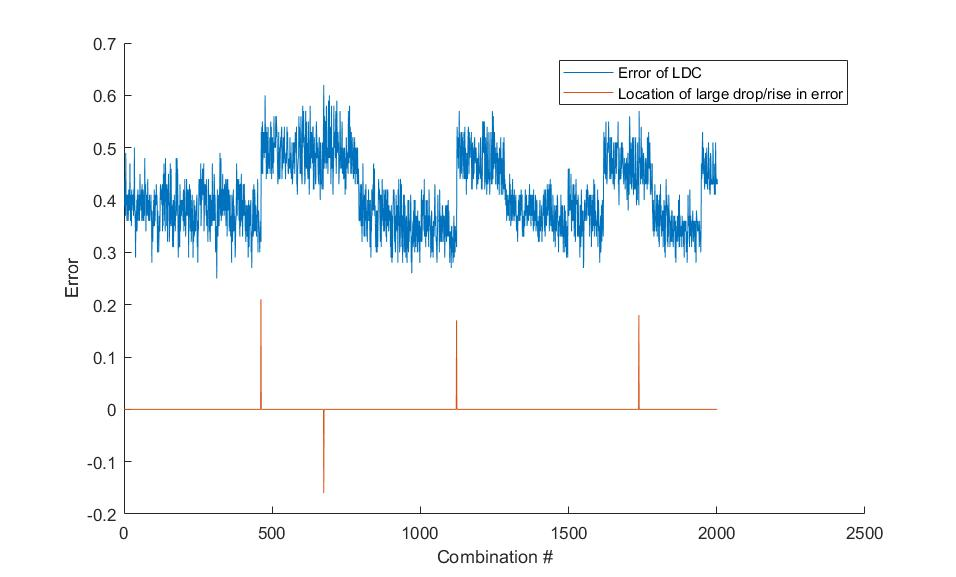
\includegraphics[scale=0.45]{images/feat_jumps.jpg}
	\caption{Error of the LDC-classifier for each possible combination of 10 out of 14 features. The orange line indicates places with a large increase or decrease in error-value.}
	\label{fig:feat_jumps}
\end{figure}
\noindent At this time, the complete system consisted of a Linear Classifier (LDC) trained on the dataset from which 10 features were selected. Sadly though, testruns of the algorithm yielded an error of 30\%. Since this was too low to meet the requirements, a different approach was taken. \\
\subsubsection*{Representation by Dissimilarity}